\chapter{Μεθοδολογία και Υλοποίηση}
\label{ch:implementation}

\section{Εισαγωγή}
\label{sec:methodology-introduction}

Στο παρόν κεφάλαιο παρουσιάζεται η μεθοδολογία που ακολουθήθηκε για την
απόσταξη γνώσης από το προεκπαιδευμένο \tl{V-JEPA Large}, το οποίο
χρησιμοποιείται ως μοντέλο-\tl{teacher}, προς μικρότερες αρχιτεκτονικές
της ίδιας οικογένειας. Ως μοντέλα-\tl{student} εξετάζονται τα
\tl{V-JEPA Base}, \tl{V-JEPA Small} και \tl{V-JEPA Tiny}, με στόχο τη
μεταφορά της γνώσης του \tl{teacher} και της ικανότητάς του να παράγει
χρήσιμες αναπαραστάσεις βίντεο.

Η πειραματική διαδικασία οργανώνεται γύρω από τρεις στρατηγικές απόσταξης
γνώσης. Η πρώτη πραγματοποιεί απόσταξη στο επίπεδο των τελικών
προβλέψεων, ενώ η δεύτερη συνδυάζει την αντιστοίχιση των τελικών
προβλέψεων με την αντιστοίχιση των ενδιάμεσων αναπαραστάσεων. Η τρίτη
στρατηγική περιορίζει την απόσταξη στο \tl{backbone} του
μοντέλου-\tl{student} και ακολουθείται από ξεχωριστό στάδιο
επιβλεπόμενης εκπαίδευσης του \tl{attentive classifier}, με τα βάρη του
αποσταγμένου \tl{backbone} να παραμένουν παγωμένα.

Η υλοποίηση των πειραμάτων πραγματοποιήθηκε στη γλώσσα προγραμματισμού
\tl{Python}, με χρήση του πλαισίου βαθιάς μάθησης (\tl{deep learning framework}) \tl{PyTorch}\cite{paszke2019pytorch} τόσο για
την επεξεργασία των δεδομένων όσο και για την εκπαίδευση
και την αξιολόγηση των μοντέλων.
\section{Φόρτωση και προετοιμασία των δεδομένων}
\label{sec:data-preparation}

\begin{figure}[H]
    \centering
    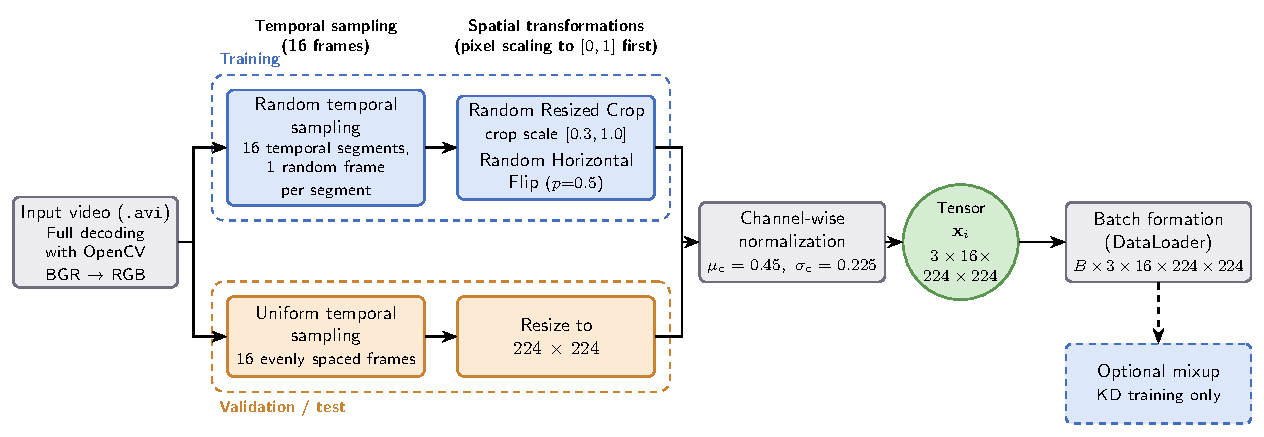
\includegraphics[width=\textwidth]{tikz/data_pipeline.pdf}
    \caption{Διαδικασία φόρτωσης και προετοιμασίας των δεδομένων. Κάθε
    βίντεο αποκωδικοποιείται πλήρως και από αυτό επιλέγονται 16 καρέ με
    διαφορετική στρατηγική για την εκπαίδευση και την επικύρωση ή τον
    έλεγχο. Μετά την εφαρμογή των χωρικών μετασχηματισμών και της
    κανονικοποίησης, κάθε απόσπασμα αναπαρίσταται ως \tl{tensor}
    \(\mathbf{x}_i\) διαστάσεων \(3\times16\times224\times224\). Τα αποσπάσματα ομαδοποιούνται μέσω του \tl{DataLoader} σε παρτίδες
    \(\mathcal{B}\), ενώ στα πειράματα απόσταξης στα οποία χρησιμοποιείται
    \tl{mixup} κάθε απόσπασμα αναμειγνύεται με ένα άλλο απόσπασμα της
    ίδιας παρτίδας (Ενότητα~\ref{subsec:batches-mixup}).}
    \label{fig:data-pipeline}
\end{figure}

Το πρώτο στάδιο της πειραματικής διαδικασίας περιλαμβάνει τη φόρτωση και
την προετοιμασία των δεδομένων πριν από την τροφοδότησή τους στα μοντέλα.
Τα μοντέλα \tl{V-JEPA} που χρησιμοποιούνται στην παρούσα εργασία
δέχονται ως είσοδο αποσπάσματα βίντεο αποτελούμενα από 16 καρέ. Επομένως,
η προετοιμασία των δεδομένων περιλαμβάνει την επιλογή των βίντεο με βάση
τον επίσημο διαχωρισμό, τον περαιτέρω διαχωρισμό του συνόλου εκπαίδευσης
σε σύνολα εκπαίδευσης και επικύρωσης (\tl{training/validation split}),
την αποκωδικοποίηση και τη χρονική δειγματοληψία των καρέ, καθώς και την
εφαρμογή των κατάλληλων χωρικών μετασχηματισμών. Η βασική αυτή διαδικασία
ακολουθείται τόσο στα πειράματα απόσταξης γνώσης όσο και στα πειράματα
επιβλεπόμενης εκπαίδευσης του \tl{attentive classifier}, με τις
επιμέρους τεχνικές επαύξησης να διαφοροποιούνται ανάλογα με την
πειραματική διαμόρφωση.


\subsection{Επιλογή και διαχωρισμός των δεδομένων}
\label{subsec:data-selection-split}

Η επιλογή των βίντεο που συμμετέχουν στον πρώτο επίσημο διαχωρισμό
(\tl{split 1}) γίνεται με βάση τα αρχεία \tl{.txt} που συνοδεύουν κάθε
σύνολο δεδομένων, τα οποία καθορίζουν την αντιστοίχιση κάθε βίντεο στο
επίσημο σύνολο εκπαίδευσης ή ελέγχου.

Για την παρακολούθηση της πορείας της εκπαίδευσης, την ανίχνευση
φαινομένων υπερεκπαίδευσης και την επιλογή του βέλτιστου μοντέλου, το
επίσημο σύνολο εκπαίδευσης κάθε συλλογής διαχωρίστηκε περαιτέρω σε ένα
εσωτερικό σύνολο εκπαίδευσης και ένα σύνολο επικύρωσης. Ο επίσημος
διαχωρισμός ελέγχου παρέμεινε ανεξάρτητος και χρησιμοποιήθηκε μόνο για
την τελική αξιολόγηση των επιλεγμένων μοντέλων. Η επιθυμητή αναλογία
μεταξύ των εσωτερικών συνόλων εκπαίδευσης και επικύρωσης ορίστηκε σε
\(80\%/20\%\).

Αρχικά, το σύνολο επικύρωσης δημιουργήθηκε με τυχαία επιλογή του
\(20\%\) των αποσπασμάτων κάθε κλάσης. Ωστόσο, και στα δύο σύνολα
δεδομένων αρκετά αποσπάσματα έχουν κοινή προέλευση. Στο \tl{HMDB51},
πολλαπλά αποσπάσματα της ίδιας κλάσης μπορεί να προέρχονται από το ίδιο
αρχικό βίντεο, ενώ στο \tl{UCF101} τα αποσπάσματα οργανώνονται σε ομάδες
(\tl{groups}), τα μέλη των οποίων παρουσιάζουν κοινά χαρακτηριστικά,
όπως το φόντο, η οπτική γωνία ή οι εικονιζόμενοι άνθρωποι
\cite{soomro2012ucf101}. Ο αρχικός τυχαίος διαχωρισμός τοποθέτησε σε
αρκετές περιπτώσεις ισχυρά συσχετισμένα αποσπάσματα τόσο στο σύνολο
εκπαίδευσης όσο και στο σύνολο επικύρωσης, προκαλώντας διαρροή δεδομένων
(\tl{data leakage}). Ως αποτέλεσμα, η επίδοση στο σύνολο επικύρωσης δεν
παρείχε αξιόπιστη εκτίμηση της ικανότητας γενίκευσης του μοντέλου σε
βίντεο διαφορετικής προέλευσης και δεν αποτελούσε κατάλληλο κριτήριο για
την επιλογή του βέλτιστου μοντέλου.

Για τον λόγο αυτό, ο διαχωρισμός πραγματοποιήθηκε τελικά σε επίπεδο
πηγής και όχι σε επίπεδο μεμονωμένου αποσπάσματος. Η πηγή κάθε
αποσπάσματος προσδιορίζεται από το όνομα του αρχείου του. Στο
\tl{HMDB51}, ως αναγνωριστικό της πηγής χρησιμοποιείται το τμήμα του
ονόματος που προηγείται της ονομασίας της κλάσης, ενώ στο \tl{UCF101}
χρησιμοποιείται ο κωδικός της ομάδας (\tl{gXX}) στην οποία ανήκει. Όλα
τα αποσπάσματα με το ίδιο αναγνωριστικό πηγής ή τον ίδιο κωδικό ομάδας
τοποθετούνται στο ίδιο σύνολο, ώστε συσχετισμένα δείγματα να μην
εμφανίζονται ταυτόχρονα στα σύνολα εκπαίδευσης και επικύρωσης. Για κάθε
κλάση, οι πηγές ανακατεύονται και προστίθενται διαδοχικά και ολόκληρες
στο σύνολο επικύρωσης, μέχρι το πλήθος των αποσπασμάτων του να
προσεγγίσει το επιθυμητό μέγεθος. Οι υπόλοιπες πηγές εντάσσονται στο
σύνολο εκπαίδευσης. Με αυτόν τον τρόπο αποτρέπεται η επικάλυψη πηγών
μεταξύ των δύο συνόλων.

Επειδή οι πηγές περιλαμβάνουν διαφορετικό αριθμό αποσπασμάτων και
διατηρούνται ακέραιες, δεν είναι πάντοτε δυνατή η επίτευξη της ακριβούς
επιθυμητής αναλογίας. Ωστόσο, όπως φαίνεται στον
Πίνακα~\ref{tab:train-validation-split}, και στα δύο σύνολα δεδομένων
προκύπτει συνολικά ένας διαχωρισμός που προσεγγίζει την αναλογία
\(80\%/20\%\).

\begin{table}[H]
    \centering
    \caption{Κατανομή των επίσημων συνόλων εκπαίδευσης μετά τη δημιουργία
    των εσωτερικών συνόλων επικύρωσης.}
    \label{tab:train-validation-split}
    \begin{tabular}{lccc}
        \hline
        \textbf{Σύνολο δεδομένων} &
        \textbf{Εκπαίδευση} &
        \textbf{Επικύρωση} &
        \textbf{Ποσοστό επικύρωσης} \\
        \hline
        \tl{HMDB51} & \(2\,876\) & \(694\)   & \(19{,}4\%\) \\
        \tl{UCF101} & \(7\,640\) & \(1\,897\) & \(19{,}9\%\) \\
        \hline
    \end{tabular}
\end{table}

Σε επίπεδο επιμέρους κλάσεων, η κατανομή των δειγμάτων στα εσωτερικά
σύνολα εκπαίδευσης και επικύρωσης δεν είναι πλήρως ισορροπημένη. Αυτό
οφείλεται στο διαφορετικό πλήθος αποσπασμάτων που περιλαμβάνει κάθε πηγή
και στην απαίτηση όλα τα αποσπάσματα κοινής προέλευσης να διατηρούνται
στο ίδιο υποσύνολο. Ως αποτέλεσμα, το \tl{HMDB51}, το επίσημο σύνολο
εκπαίδευσης του οποίου είναι αρχικά ισορροπημένο ως προς τις κλάσεις,
παρουσιάζει ανισορροπία μετά τον εσωτερικό διαχωρισμό. Αντίστοιχα, στο
\tl{UCF101} η ανισορροπία που υπάρχει ήδη στο επίσημο σύνολο
εκπαίδευσης διατηρείται και στα υποσύνολα που προκύπτουν.

Η ανισορροπία αυτή λαμβάνεται υπόψη κατά τον καθορισμό του κριτηρίου
επιλογής των μοντέλων. Ειδικότερα, όπως περιγράφεται στις ρυθμίσεις
εκπαίδευσης (Ενότητα~\ref{subsec:training-settings}), στην τελική
πειραματική διαμόρφωση της επιβλεπόμενης εκπαίδευσης των
\tl{attentive classifiers}, το βέλτιστο \tl{checkpoint} επιλέγεται με
βάση τη μέγιστη ισορροπημένη ακρίβεια στο σύνολο επικύρωσης
(Ενότητα~\ref{subsec:balanced-accuracy}), ώστε όλες οι κλάσεις να
συνεισφέρουν ισότιμα στο κριτήριο επιλογής.


\subsection{Αποκωδικοποίηση και χρονική δειγματοληψία των \tl{frames}}
\label{subsec:frame-decoding-sampling}

Κάθε επιλεγμένο βίντεο αποκωδικοποιείται ολόκληρο, καρέ προς καρέ, με
τη βιβλιοθήκη \tl{OpenCV}\cite{bradski2000opencv}. Καθώς η βιβλιοθήκη αυτή επιστρέφει τα αποκωδικοποιημένα καρέ με
διάταξη χρωματικών καναλιών \tl{BGR}, αυτά μετατρέπονται στη συνέχεια σε
\tl{RGB} πριν από την εφαρμογή των υπόλοιπων σταδίων προεπεξεργασίας. Στη συνέχεια, μέσω χρονικής δειγματοληψίας
σχηματίζεται ένα απόσπασμα μήκους 16 καρέ, το οποίο χρησιμοποιείται ως
είσοδος του μοντέλου.

Για τα δεδομένα εκπαίδευσης, η χρονική δειγματοληψία πραγματοποιείται
χωρίζοντας τη διάρκεια κάθε βίντεο σε 16 ομοιόμορφα κατανεμημένα χρονικά
τμήματα και επιλέγοντας τυχαία ένα καρέ από καθένα από αυτά. Με αυτόν τον τρόπο, τα επιλεγμένα καρέ καλύπτουν ολόκληρη τη χρονική
έκταση του βίντεο, ενώ η τυχαία επιλογή τους πραγματοποιείται εκ νέου σε
κάθε εποχή εκπαίδευσης, παράγοντας διαφορετικά αποσπάσματα από το ίδιο
βίντεο και λειτουργώντας ως μορφή χρονικής επαύξησης των δεδομένων. Αντίθετα, για τα δεδομένα επικύρωσης και ελέγχου
επιλέγονται 16 καρέ ομοιόμορφα κατανεμημένα σε ολόκληρη τη χρονική
διάρκεια του βίντεο, ώστε η διαδικασία αξιολόγησης να είναι
ντετερμινιστική.


\subsection{Χωρικοί μετασχηματισμοί και επαύξηση των δεδομένων}
\label{subsec:transform-data-augmentations}

Πριν από την είσοδό τους στο μοντέλο, οι τιμές των \tl{pixels} των καρέ
μετασχηματίζονται ώστε να ανοίκουν στο διάστημα \([0,1]\). Στα δεδομένα εκπαίδευσης, για τα
πειράματα στα οποία εφαρμόζονται τεχνικές χωρικής επαύξησης,
χρησιμοποιείται τυχαία περικοπή και αλλαγή μεγέθους
(\tl{Random Resized Crop}). Ειδικότερα, επιλέγεται τυχαία μια περιοχή
που καλύπτει από το \(30\%\) έως το \(100\%\) της επιφάνειας του αρχικού
καρέ, με αναλογία διαστάσεων μεταξύ \(3/4\) και \(4/3\), η οποία στη
συνέχεια μετατρέπεται σε ανάλυση \(224\times224\). Επιπλέον, εφαρμόζεται
τυχαία οριζόντια αναστροφή (\tl{Random Horizontal Flip}) με πιθανότητα
\(p=0{,}5\). Οι μετασχηματισμοί αυτοί υλοποιούνται μέσω της βιβλιοθήκης
\tl{torchvision} και εφαρμόζονται σε ολόκληρο το απόσπασμα με τις ίδιες
τυχαία επιλεγμένες παραμέτρους για όλα τα καρέ, ώστε να διατηρείται η
χρονική τους συνοχή.

Στα δεδομένα επικύρωσης και ελέγχου δεν εφαρμόζονται τυχαίες επαυξήσεις.
Τα καρέ μετατρέπονται απευθείας σε ανάλυση \(224\times224\), ώστε να
διατηρείται ολόκληρο το οπτικό τους πεδίο.

Μετά την εφαρμογή των χωρικών μετασχηματισμών, οι τιμές των
\tl{pixels} κανονικοποιούνται ανά χρωματικό κανάλι \(c\) σύμφωνα με τη
σχέση:

\begin{equation}
    \hat{x}_c = \frac{x_c-\mu_c}{\sigma_c},
\end{equation}

όπου \(\mu_c=0{,}45\) και \(\sigma_c=0{,}225\) για καθένα από τα τρία
χρωματικά κανάλια. Οι τιμές αυτές αποτελούν συνήθη διαμόρφωση
κανονικοποίησης σε εφαρμογές αναγνώρισης βίντεο, όπως στην υλοποίηση
\tl{PySlowFast} \cite{fan2020pyslowfast}, και διατηρήθηκαν σταθερές σε
όλα τα πειράματα.


% Προηγούμενη εκδοχή του σχήματος (δύο εφαρμογές του Random Resized Crop, κλάση clap):
% \begin{figure}[H]
%     \centering
%     \includegraphics[width=\textwidth]
%     {random_resized_crop_example.pdf}
%     \caption{Παράδειγμα δύο τυχαίων εφαρμογών του
% \tl{Random Resized Crop} στα ίδια καρέ ενός βίντεο της κλάσης
% \tl{clap} από το \tl{HMDB51}. Στην επάνω σειρά σημειώνονται οι δύο
% τυχαία επιλεγμένες περιοχές και στις επόμενες σειρές παρουσιάζονται τα
% αντίστοιχα αποτελέσματα. Οι παράμετροι της περικοπής επιλέγονται εκ νέου
% σε κάθε εποχή εκπαίδευσης, αλλά εφαρμόζονται με τον ίδιο τρόπο σε όλα τα
% καρέ κάθε αποσπάσματος, ώστε να διατηρείται η χρονική τους συνοχή.}
% \end{figure}

\begin{figure}[H]
    \centering
    \includegraphics[width=\textwidth]
    {random_resized_crop_flip_example.pdf}
    \caption{Παράδειγμα εφαρμογής των χωρικών επαυξήσεων σε τέσσερα από τα
    \(16\) δειγματοληπτημένα καρέ ενός βίντεο της κλάσης \tl{pour} από το
    \tl{HMDB51}. Στην επάνω σειρά οριοθετείται με πλαίσιο η περιοχή που
επιλέχθηκε τυχαία για το \tl{Random Resized Crop}, στη μεσαία σειρά
παρουσιάζεται το αποτέλεσμα της περικοπής και της αλλαγής μεγέθους σε
\(224\times224\), ενώ στην κάτω σειρά παρουσιάζεται το ίδιο αποτέλεσμα
μετά την εφαρμογή οριζόντιας αναστροφής. Οι παράμετροι επιλέγονται εκ
    νέου σε κάθε εποχή εκπαίδευσης.}

\end{figure}


\subsection{Σχηματισμός παρτίδων και εφαρμογή του \tl{mixup}}
\label{subsec:batches-mixup}

Μετά την ολοκλήρωση της προεπεξεργασίας, κάθε απόσπασμα βίντεο
αναπαρίσταται ως \tl{tensor} διαστάσεων
\(C\times T\times H\times W=3\times16\times224\times224\), όπου \(C\)
είναι το πλήθος των χρωματικών καναλιών, \(T\) το πλήθος των καρέ και
\(H\), \(W\) το ύψος και το πλάτος κάθε καρέ, αντίστοιχα. Τα δείγματα
ομαδοποιούνται στη συνέχεια σε παρτίδες (\tl{batches}) με την κλάση
\tl{DataLoader} της βιβλιοθήκης \tl{PyTorch}, για τη μαζική επεξεργασία
τους κατά τα στάδια εκπαίδευσης, επικύρωσης και ελέγχου. Κατά την
εκπαίδευση, η σειρά των δειγμάτων ανακατεύεται (\tl{shuffling}) σε κάθε εποχή πριν από
τον σχηματισμό των παρτίδων , ενώ κατά την επικύρωση και τον έλεγχο
διατηρείται σταθερή.

Στα πειράματα απόσταξης γνώσης στα οποία χρησιμοποιείται η τεχνική
\tl{mixup}, ακολουθείται η προσέγγιση των \tl{Beyer et al.}
\cite{beyer2022knowledge}. Για κάθε παρτίδα μεγέθους \(B\), επιλέγεται
ένας συντελεστής \(\lambda\) από την ομοιόμορφη κατανομή
\(\mathcal{U}(0,1)\), κοινός για όλα τα δείγματα της παρτίδας. Στην
υλοποίηση της παρούσας εργασίας, κάθε απόσπασμα \(\mathbf{x}_i\)
αναμειγνύεται με το προηγούμενο απόσπασμα της ίδιας παρτίδας
\(\mathbf{x}_j\), σύμφωνα με τη σχέση:

\begin{equation}
    \widetilde{\mathbf{x}}_i
    =
    \lambda\mathbf{x}_i+
    (1-\lambda)\mathbf{x}_j,
\end{equation}
Καθώς η σειρά των δειγμάτων ανακατεύεται εκ νέου σε κάθε εποχή, τα
ζεύγη που αναμειγνύονται μεταβάλλονται μεταξύ των εποχών. Για κάθε
ζεύγος αποσπασμάτων, ο ίδιος συντελεστής \(\lambda\) εφαρμόζεται σε όλα
τα αντίστοιχα καρέ, ώστε η ανάμειξη να παραμένει συνεπής σε ολόκληρη τη
χρονική διάσταση, όπως φαίνεται στο
Σχήμα~\ref{fig:mixup-example}.

Η ίδια αναμεμειγμένη είσοδος παρέχεται στα
μοντέλα-\tl{teacher} και \tl{student}, ώστε η αντιστοίχιση των εξόδων ή
των αναπαραστάσεών τους να πραγματοποιείται για το ίδιο επαυξημένο
δείγμα.

\begin{figure}[H]
    \centering
    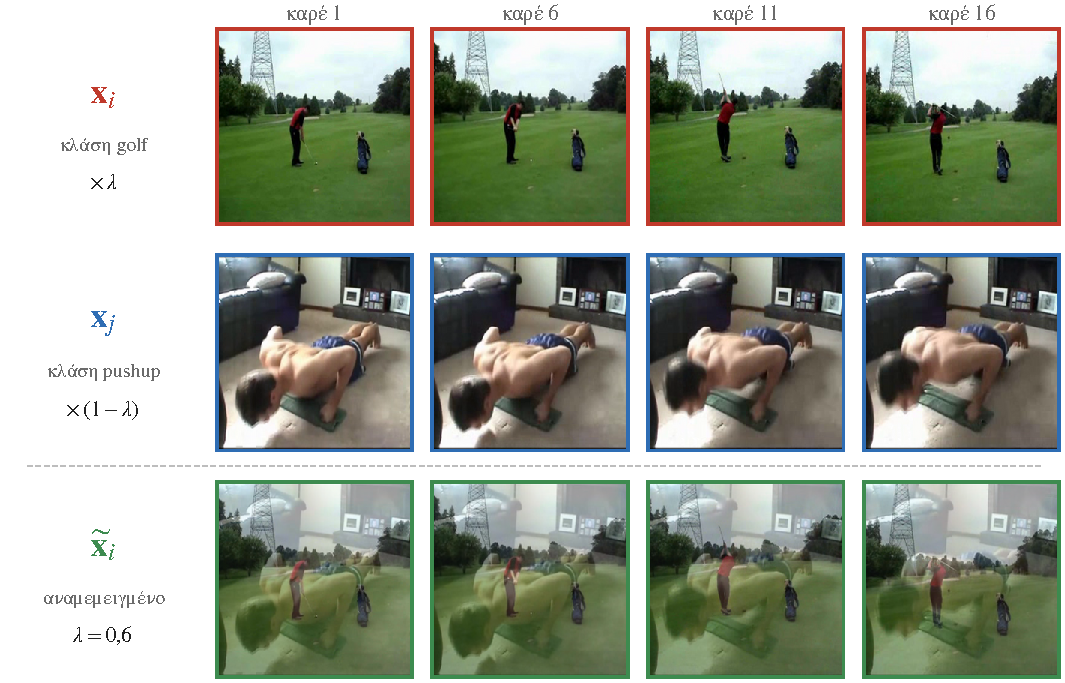
\includegraphics[width=\textwidth]{mixup_example.pdf}
    \caption{Παράδειγμα εφαρμογής του \tl{mixup} σε δύο αποσπάσματα του
    \tl{HMDB51} για \(\lambda=0{,}6\). Παρουσιάζονται τέσσερα ενδεικτικά
καρέ από τα 16 δειγματοληπτημένα καρέ κάθε αποσπάσματος. Η μίξη πραγματοποιείται με το ίδιο
    \(\lambda\) σε όλα τα καρέ, ενώ το αναμεμειγμένο απόσπασμα
    \(\widetilde{\mathbf{x}}_i\) τροφοδοτείται τόσο στον \tl{teacher} όσο
    και στον \tl{student}.}
    \label{fig:mixup-example}
\end{figure}

\section{Μοντέλα αναφοράς}
\label{sec:baseline-models}

Πριν από την παρουσίαση των στρατηγικών απόσταξης, είναι σημαντικό να
εξεταστεί η απόδοση που επιτυγχάνουν τα μοντέλα-\tl{student} όταν
εκπαιδεύονται αποκλειστικά με επιβλεπόμενο τρόπο στο \tl{HMDB51}, χωρίς
καθοδήγηση από το μοντέλο-\tl{teacher}. Τα μοντέλα αυτά αποτελούν το
σημείο αναφοράς (\tl{supervised baselines}) για την αξιολόγηση των
στρατηγικών απόσταξης, καθώς η σύγκρισή τους με τα αντίστοιχα
αποσταγμένα μοντέλα επιτρέπει να εκτιμηθεί η επίδραση της απόσταξης
γνώσης στην τελική τους απόδοση.

Για καθεμία από τις αρχιτεκτονικές \tl{V-JEPA Base}, \tl{Small} και
\tl{Tiny}, το \tl{backbone} αρχικοποιείται με τυχαία βάρη και
εκπαιδεύεται από άκρο σε άκρο μαζί με τον αντίστοιχο \tl{attentive classifier}.
Η εκπαίδευση πραγματοποιείται με βάση τις πραγματικές ετικέτες των
κλάσεων, χρησιμοποιώντας τη συνάρτηση απώλειας \tl{cross-entropy} με
εξομάλυνση ετικετών (\tl{label smoothing}) ίση με \(0{,}1\). Για τη διατήρηση συγκρίσιμων συνθηκών, χρησιμοποιούνται ο ίδιος
εσωτερικός διαχωρισμός των δεδομένων και η ίδια βασική διαδικασία
χρονικής δειγματοληψίας και χωρικής προεπεξεργασίας με τα πειράματα
απόσταξης. Οι υπερπαράμετροι εκπαίδευσης προσαρμόζονται στην αντίστοιχη
πειραματική διαμόρφωση και παρουσιάζονται αναλυτικά στην
Ενότητα~\ref{sec:training-implementation-settings}.

\section{Στρατηγικές απόσταξης γνώσης}
\label{sec:distillation-strategies}

Οι στρατηγικές απόσταξης γνώσης που εξετάζονται στην παρούσα εργασία
διαμορφώθηκαν αρχικά με βάση ιδέες από τη δημοσίευση
\tl{Knowledge Distillation: A Good Teacher is Patient and Consistent}
\cite{beyer2022knowledge}. Ειδικότερα, υιοθετήθηκαν η παροχή της ίδιας
επαυξημένης εισόδου στα μοντέλα-\tl{teacher} και \tl{student}, η
αξιοποίηση της τεχνικής \tl{mixup} στα περισσότερα πειράματα, καθώς και
η εκπαίδευση για μεγάλο αριθμό εποχών, με στόχο την αποτελεσματικότερη
μεταφορά της γνώσης. Στη συνέχεια, λόγω της φύσης του \tl{V-JEPA} ως
μοντέλου εκμάθησης αναπαραστάσεων, εξετάστηκαν δύο επιπλέον στρατηγικές:
ο συνδυασμός της απόσταξης των τελικών προβλέψεων του
\tl{attentive classifier} με την απόσταξη των αναπαραστάσεων του
\tl{backbone}, καθώς και η απόσταξη αποκλειστικά των αναπαραστάσεων
αυτών. Η σύγκριση των τριών στρατηγικών απεικονίζεται στο
Σχήμα~\ref{fig:kd-overview}.

\begin{figure}[H]
    \vspace{\baselineskip}
    \centering
    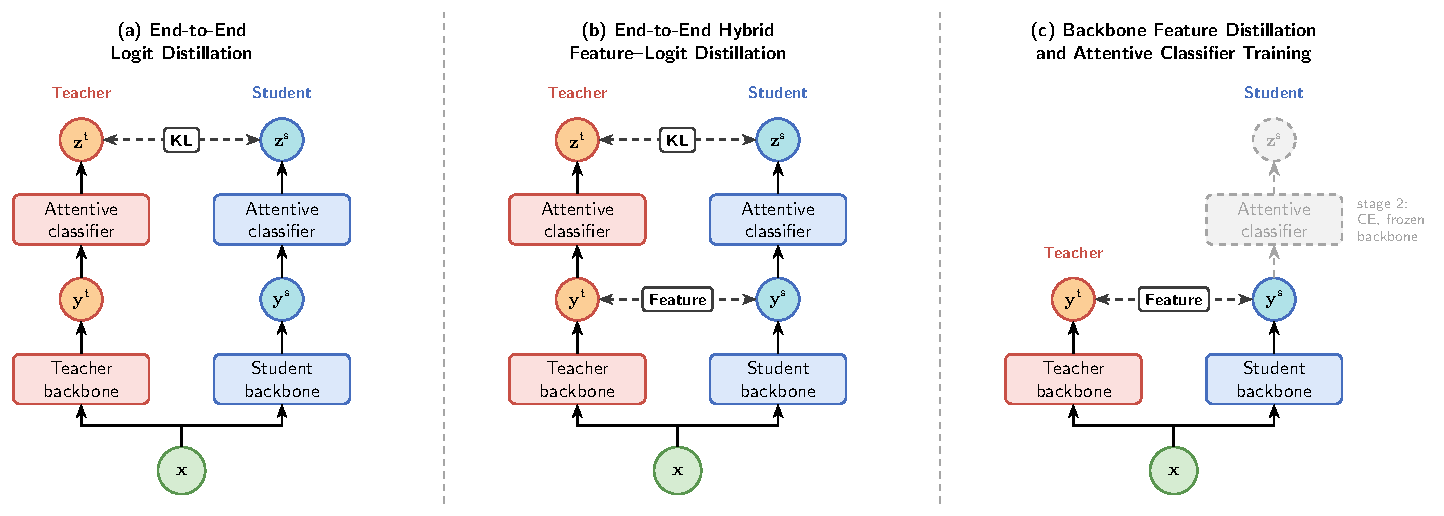
\includegraphics[width=\textwidth]{tikz/kd_overview.pdf}
    \caption{Συνοπτική σύγκριση των τριών στρατηγικών απόσταξης γνώσης.
    Τα διακεκομμένα βέλη υποδεικνύουν τα σημεία στα οποία εφαρμόζεται η
    απόσταξη: στα \tl{logits} \(\mathbf{z}\) μέσω της απόκλισης \tl{KL},
    στις αναπαραστάσεις \(\mathbf{y}\) των \tl{backbones}, ή και στα δύο.
    Στην τρίτη στρατηγική, ο \tl{attentive classifier} του \tl{student}
    εκπαιδεύεται σε ξεχωριστό, δεύτερο στάδιο.}
    \label{fig:kd-overview}
\end{figure}

Ως μοντέλο-\tl{teacher} χρησιμοποιήθηκε το \tl{V-JEPA Large backbone} με
τα επίσημα προεκπαιδευμένα βάρη του, σε συνδυασμό με έναν
\tl{attentive classifier}, ο οποίος εκπαιδεύτηκε με επιβλεπόμενο τρόπο
στο \tl{HMDB51}. Κατά την εκπαίδευση του ταξινομητή, οι παράμετροι του
\tl{backbone} παρέμειναν παγωμένες και ενημερώθηκαν μόνο οι παράμετροι
του \tl{attentive classifier}. Μετά την ολοκλήρωση του σταδίου αυτού,
τα δύο τμήματα αποτέλεσαν από κοινού το μοντέλο-\tl{teacher} που
χρησιμοποιήθηκε στα πειράματα απόσταξης.

Σε όλα τα πειράματα απόσταξης, οι παράμετροι του
μοντέλου-\tl{teacher} παραμένουν παγωμένες. Ανάλογα με τη στρατηγική,
ως στόχοι εκπαίδευσης χρησιμοποιούνται είτε οι ενδιάμεσες αναπαραστάσεις
που παράγει το \tl{backbone} είτε τα \tl{logits} του
\tl{attentive classifier}, είτε ο συνδυασμός τους. Αντίθετα, τα βάρη του μοντέλου-\tl{student} αρχικοποιούνται τυχαία και
ενημερώνονται κατά τη διάρκεια της εκπαίδευσης, ώστε οι έξοδοί του να
προσεγγίζουν τις αντίστοιχες εξόδους του μοντέλου-\tl{teacher}.

\subsection{Απόσταξη τελικών προβλέψεων πλήρους μοντέλου
(\tl{End-to-End Logit Distillation})}
\label{subsec:full-model-distillation}

Η πρώτη στρατηγική αφορά την απόσταξη γνώσης στις τελικές προβλέψεις του
μοντέλου-\tl{teacher}. Για κάθε απόσπασμα βίντεο, το
μοντέλο-\tl{student} εκπαιδεύεται ώστε να προσεγγίζει την κατανομή
πιθανοτήτων που παράγει το μοντέλο-\tl{teacher} για τις κλάσεις ενεργειών
του \tl{HMDB51}, ελαχιστοποιώντας την απόκλιση
\tl{Kullback--Leibler} μεταξύ των δύο κατανομών. Σε όλα τα πειράματα της
συγκεκριμένης στρατηγικής, η παράμετρος θερμοκρασίας διατηρείται σταθερή
σε \(T=1\). Η διαδικασία απεικονίζεται στο
Σχήμα~\ref{fig:kd-full-model}.

Το μοντέλο-\tl{student} αποτελείται από ένα
μικρότερο \tl{V-JEPA backbone} και έναν νέο
\tl{attentive classifier}, τα οποία εκπαιδεύονται από κοινού και από
άκρο σε άκρο.  Οι πραγματικές ετικέτες
των δεδομένων δεν συμμετέχουν στη συνάρτηση απώλειας και, επομένως, δεν
καθοδηγούν άμεσα την ενημέρωση των παραμέτρων του \tl{student}.
Χρησιμοποιούνται μόνο για τον υπολογισμό των μετρικών και την επιλογή
του βέλτιστου \tl{checkpoint} στο σύνολο επικύρωσης.

\begin{figure}[H]
    \centering
    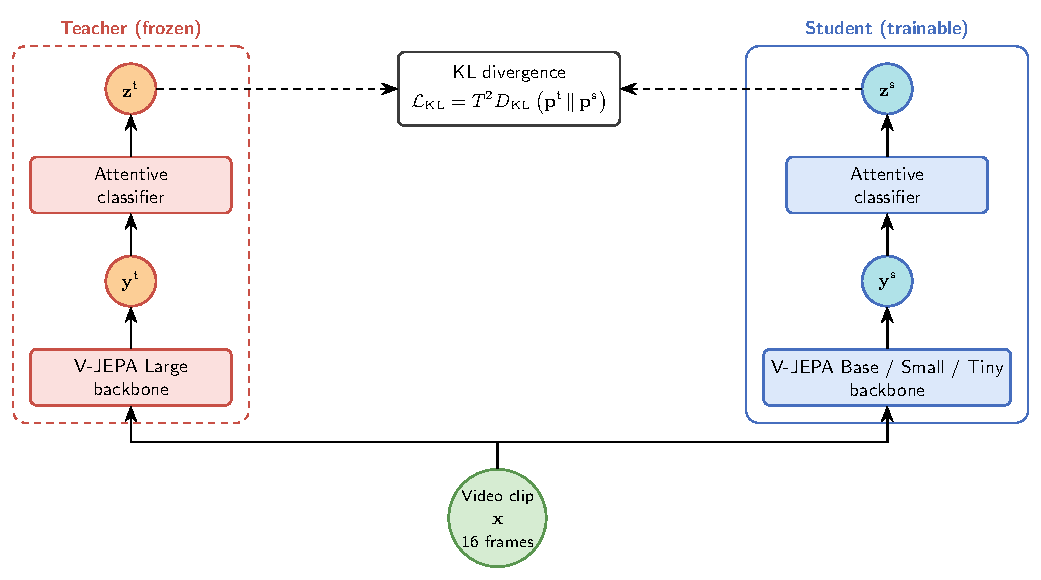
\includegraphics[width=\textwidth]{tikz/kd_full_model.pdf}
    \caption{Απόσταξη τελικών προβλέψεων πλήρους μοντέλου. Το ίδιο απόσπασμα \(\mathbf{x}\)
    τροφοδοτείται στον \tl{teacher} και στον \tl{student}. Τα
    \(\mathbf{y}^{\mathrm{t}}\) και \(\mathbf{y}^{\mathrm{s}}\) είναι οι
    αναπαραστάσεις των \tl{backbones} και τα \(\mathbf{z}^{\mathrm{t}}\) και
    \(\mathbf{z}^{\mathrm{s}}\) τα \tl{logits} των \tl{attentive classifiers}.
    Ο \tl{student} εκπαιδεύεται ελαχιστοποιώντας την απόκλιση \tl{KL} μεταξύ
    των κατανομών
    \(\mathbf{p}^{\mathrm{t}}=\operatorname{softmax}(\mathbf{z}^{\mathrm{t}}/T)\)
    και
    \(\mathbf{p}^{\mathrm{s}}=\operatorname{softmax}(\mathbf{z}^{\mathrm{s}}/T)\).}
    \label{fig:kd-full-model}
\end{figure}

Η στρατηγική εφαρμόστηκε στις αρχιτεκτονικές \tl{V-JEPA Base},
\tl{Small} και \tl{Tiny} για 100 εποχές χωρίς χρήση \tl{mixup},
ενώ επίσης πραγματοποιήθηκε μία παραλλαγή για την αρχιτεκτονική
\tl{Tiny} με χρήση \tl{mixup}, στην οποία η ίδια αναμεμειγμένη είσοδος
παρέχεται στα μοντέλα-\tl{teacher} και \tl{student}.

\subsection{Υβριδική απόσταξη γνώσης
(\tl{End-to-End Hybrid Feature--Logit Distillation})}
\label{subsec:hybrid-distillation}

Η δεύτερη στρατηγική συνδυάζει την απόσταξη των τελικών προβλέψεων με
την αντιστοίχιση των αναπαραστάσεων που παράγουν τα \tl{backbones} των
δύο μοντέλων. Επομένως, ο \tl{student} καθοδηγείται τόσο από τα
\tl{logits} του \tl{teacher} όσο και από τις αναπαραστάσεις του, μέσω
του σταθμισμένου συνδυασμού των δύο αντίστοιχων όρων απώλειας. Οι
αναπαραστάσεις αυτές αποτελούν τις εξόδους των δύο \tl{backbones} πριν
από τους αντίστοιχους \tl{attentive classifiers}.

Η πρώτη συνιστώσα της συνάρτησης απώλειας είναι η απόκλιση
\tl{Kullback--Leibler}, η οποία, όπως και στην πρώτη στρατηγική,
εφαρμόζεται στις κατανομές πιθανοτήτων που προκύπτουν από τα \tl{logits}
των δύο μοντέλων. Η δεύτερη συνιστώσα αντιστοιχίζει τις αναπαραστάσεις που παράγουν τα
δύο \tl{backbones}. Για την αντιστοίχιση αυτή εξετάστηκαν το μέσο
τετραγωνικό σφάλμα (\tl{MSE}) και η συνάρτηση \tl{SmoothL1}
(Εξισώσεις~\eqref{eq:mse-loss} και~\eqref{eq:smooth-l1-loss}).

Κάθε αναπαράσταση \tl{token} του \tl{teacher} έχει διάσταση
\(D_T=1024\), ενώ η αντίστοιχη διάσταση \(D_S\) του \tl{student} είναι
\(768\), \(384\) και \(192\) για τις αρχιτεκτονικές \tl{V-JEPA Base},
\tl{Small} και \tl{Tiny}, αντίστοιχα. Για να καταστεί δυνατή η σύγκρισή
τους, μετά την έξοδο του \tl{backbone} του \tl{student} προστίθεται ένας
εκπαιδεύσιμος γραμμικός προβολέας (\tl{linear projector})

\[
P_S:\mathbb{R}^{D_S}\rightarrow\mathbb{R}^{D_T},
\]

ο οποίος προβάλλει τις αναπαραστάσεις του \tl{student} στη διάσταση των
αντίστοιχων αναπαραστάσεων του \tl{teacher}. Καθώς η έξοδος κάθε
\tl{backbone} περιλαμβάνει μία αναπαράσταση για κάθε \tl{token}, ο
προβολέας εφαρμόζεται ανεξάρτητα στην αναπαράσταση κάθε \tl{token} του
\tl{student}. Η απώλεια υπολογίζεται στη συνέχεια μεταξύ των προβεβλημένων
αναπαραστάσεων του \tl{student} και των αντίστοιχων αναπαραστάσεων του
\tl{teacher}:
\begin{equation}
    \mathcal{L}_{\mathrm{feat}}
    =
    \ell\left(P_S\left(\mathbf{y}^{\mathrm{s}}\right),
    \mathbf{y}^{\mathrm{t}}\right),
    \label{eq:feat-loss}
\end{equation}
όπου τα \(\mathbf{y}^{\mathrm{s}}\) και \(\mathbf{y}^{\mathrm{t}}\)
είναι οι τανυστές εξόδου των δύο \tl{backbones} και περιλαμβάνουν τις
αναπαραστάσεις όλων των \tl{tokens}, ενώ \(\ell\) είναι είτε η συνάρτηση
\tl{MSE} είτε η \tl{SmoothL1}. Ο προβολέας χρησιμοποιείται μόνο για τον υπολογισμό της
απώλειας αναπαραστάσεων, ενώ ο \tl{attentive classifier} του
\tl{student} δέχεται απευθείας τις αρχικές αναπαραστάσεις του δικού του
\tl{backbone}.

Η συνολική συνάρτηση απώλειας ορίζεται ως το σταθμισμένο άθροισμα των
δύο συνιστωσών:
\begin{equation}
    \mathcal{L}_{\mathrm{hybrid}}
    =
    \lambda_{\mathrm{KL}}\mathcal{L}_{\mathrm{KL}}
    +
    \lambda_{\mathrm{feat}}\mathcal{L}_{\mathrm{feat}},
    \label{eq:hybrid-loss}
\end{equation}
όπου οι συντελεστές \(\lambda_{\mathrm{KL}}\) και
\(\lambda_{\mathrm{feat}}\) καθορίζουν τη συνεισφορά κάθε όρου. Με βάση την απώλεια αυτή
ενημερώνονται από κοινού οι παράμετροι του \tl{student backbone}, του
\tl{attentive classifier} και του προβολέα, ενώ οι παράμετροι του
\tl{teacher} παραμένουν παγωμένες. Η διαδικασία απεικονίζεται στο
Σχήμα~\ref{fig:kd-hybrid}.

\begin{figure}[H]
    \centering
    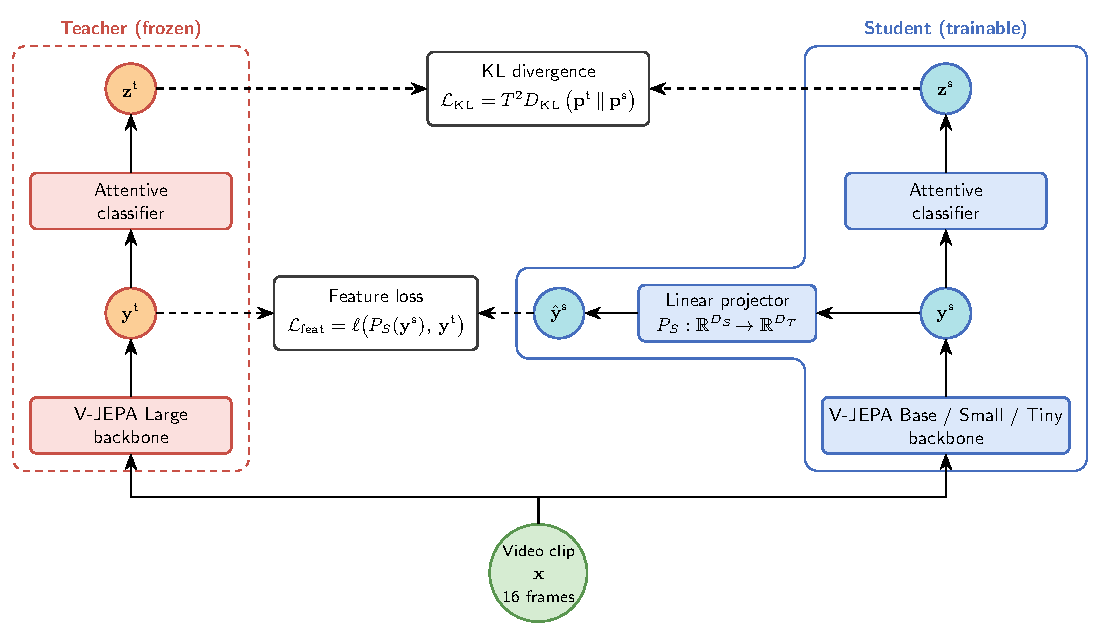
\includegraphics[width=\textwidth]{tikz/kd_hybrid.pdf}
    \caption{Υβριδική απόσταξη γνώσης. Εκτός από την απόκλιση \tl{KL}
    μεταξύ των κατανομών
    \(\mathbf{p}^{\mathrm{t}}=\operatorname{softmax}(\mathbf{z}^{\mathrm{t}}/T)\)
    και
    \(\mathbf{p}^{\mathrm{s}}=\operatorname{softmax}(\mathbf{z}^{\mathrm{s}}/T)\),
    ο \tl{student} εκπαιδεύεται ώστε η
    προβεβλημένη αναπαράστασή του
    \(\hat{\mathbf{y}}^{\mathrm{s}} = P_S(\mathbf{y}^{\mathrm{s}})\) να
    προσεγγίζει την αναπαράσταση \(\mathbf{y}^{\mathrm{t}}\) του
    \tl{teacher}. Ο προβολέας \(P_S\) χρησιμοποιείται μόνο για τον
    υπολογισμό της απώλειας αναπαραστάσεων.}
    \label{fig:kd-hybrid}
\end{figure}

Πέρα από τον απλό γραμμικό προβολέα, εξετάστηκαν τρεις εναλλακτικές
διαμορφώσεις: ένας γραμμικός προβολέας ακολουθούμενος από
\tl{LayerNorm}, ένας μη γραμμικός προβολέας και η αντίστροφη προβολή.
Ο μη γραμμικός προβολέας αποτελείται από δύο γραμμικά επίπεδα, με
κανονικοποίηση \tl{LayerNorm} μετά από καθένα από αυτά και συνάρτηση
ενεργοποίησης \tl{GELU} (\tl{Gaussian Error Linear Unit})
\cite{hendrycks2016gaussian} μεταξύ τους. Η συνάρτηση αυτή ορίζεται ως
\(\operatorname{GELU}(x)=x\,\Phi(x)\), όπου \(\Phi\) είναι η αθροιστική
συνάρτηση κατανομής της τυπικής κανονικής κατανομής, και χρησιμοποιείται
ευρέως στις αρχιτεκτονικές \tl{Vision Transformer}
\cite{dosovitskiy2021image}. Στην αντίστροφη προβολή, οι αναπαραστάσεις
του \tl{teacher} μετασχηματίζονται στη διάσταση του αντίστοιχου
\tl{student} μέσω ενός προβολέα που εφαρμόζεται στην έξοδο του
\tl{teacher backbone}, το οποίο παραμένει παγωμένο. Σε όλες τις
διαμορφώσεις, οι παράμετροι του προβολέα είναι εκπαιδεύσιμες και
ενημερώνονται μαζί με τις παραμέτρους του \tl{student}.

Επιπλέον, εξετάστηκαν διαφορετικές τιμές του συντελεστή
\(\lambda_{\mathrm{feat}}\), της παραμέτρου θερμοκρασίας \(T\) και της διάρκειας
εκπαίδευσης, οι οποίες παρουσιάζονται μαζί με τα αποτελέσματα στο
Κεφάλαιο~\ref{ch:experiments}.

Η λογική της στρατηγικής αυτής έγκειται στη συμπληρωματική πληροφορία
που παρέχουν οι δύο μορφές καθοδήγησης. Τα \tl{logits} αποτυπώνουν την
τελική εκτίμηση του \tl{teacher} για τις διαφορετικές κλάσεις, ενώ οι
αναπαραστάσεις του \tl{backbone} κωδικοποιούν πληροφορία για το
χωροχρονικό περιεχόμενο του βίντεο πριν από την τελική ταξινόμηση.
Επομένως, ο \tl{student} καθοδηγείται τόσο ως προς την τελική πρόβλεψη
όσο και ως προς τον τρόπο αναπαράστασης της εισόδου.

\subsection{Απόσταξη του \tl{backbone} και εκπαίδευση του
\tl{attentive classifier} (\tl{Backbone Feature Distillation and Attentive Classifier Training})}
\label{subsec:backbone-distillation}

Η τρίτη στρατηγική ακολουθεί μια διαδικασία δύο σταδίων, στην οποία η
εκμάθηση των αναπαραστάσεων διαχωρίζεται από την εκπαίδευση του
ταξινομητή. Η διαδικασία απεικονίζεται στο Σχήμα~\ref{fig:kd-two-stage}.

\begin{figure}[H]
    \centering
    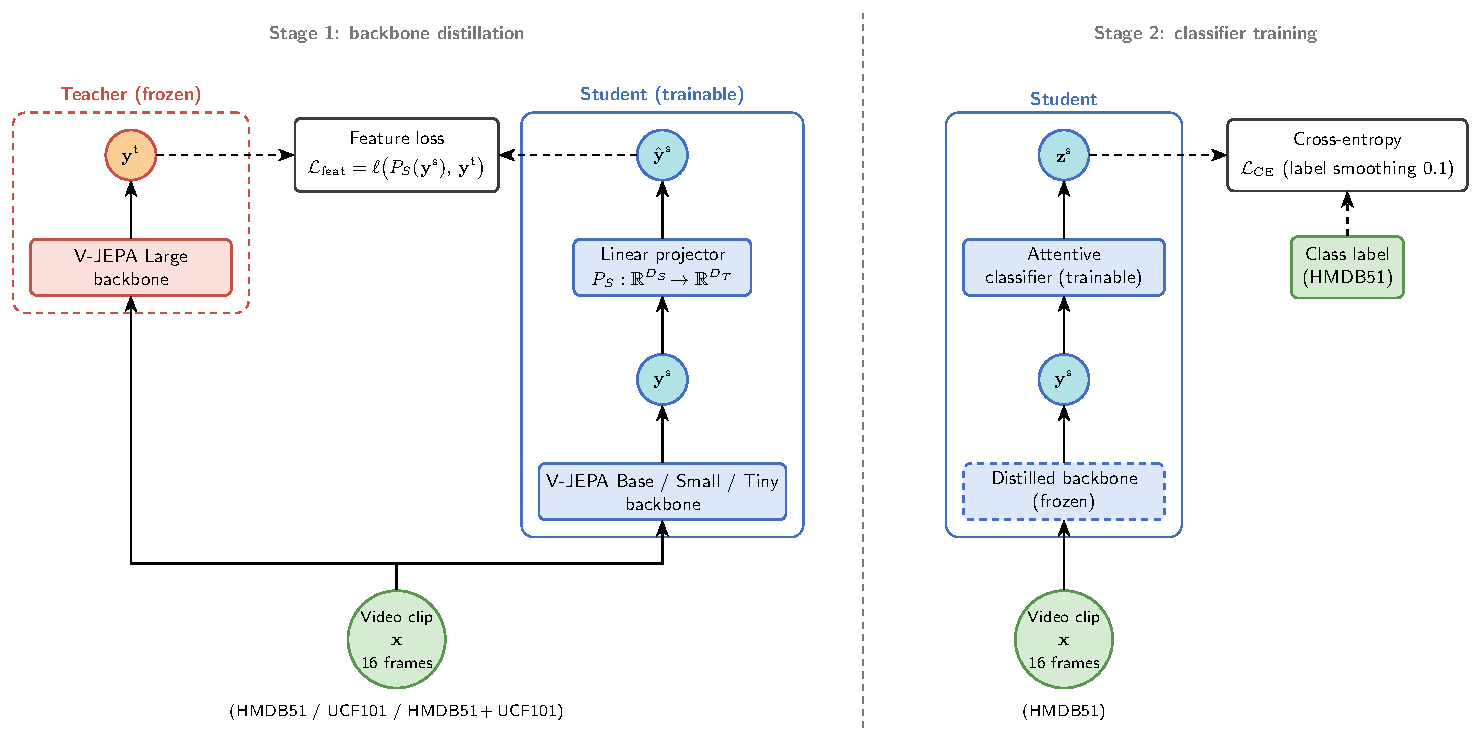
\includegraphics[width=\textwidth]{tikz/kd_two_stage.pdf}
    \caption{Απόσταξη γνώσης δύο σταδίων. Στο πρώτο στάδιο, το
    \tl{student backbone} εκπαιδεύεται ώστε οι προβεβλημένες αναπαραστάσεις
    του \(\hat{\mathbf{y}}^{\mathrm{s}} =
    P_S(\mathbf{y}^{\mathrm{s}})\) να προσεγγίζουν τις αντίστοιχες
    αναπαραστάσεις \(\mathbf{y}^{\mathrm{t}}\) του \tl{teacher backbone},
    χωρίς τη χρήση ετικετών. Στο δεύτερο στάδιο, ο προβολέας απορρίπτεται,
    το αποσταγμένο \tl{backbone} παραμένει παγωμένο και εκπαιδεύεται ένας
    \tl{attentive classifier} με συνάρτηση απώλειας
    \tl{cross-entropy}.}
    \label{fig:kd-two-stage}
\end{figure}

Στο πρώτο στάδιο, το \tl{backbone} του \tl{student} εκπαιδεύεται ώστε οι
αναπαραστάσεις του να προσεγγίζουν τις αντίστοιχες αναπαραστάσεις του
\tl{teacher backbone}. Όπως και στην υβριδική στρατηγική, οι
αναπαραστάσεις του \tl{student} προβάλλονται στη διάσταση του
\tl{teacher} μέσω ενός εκπαιδεύσιμου γραμμικού προβολέα \(P_S\), και η
απώλεια υπολογίζεται μεταξύ των αναπαραστάσεων των αντίστοιχων
\tl{tokens}, σύμφωνα με την Εξίσωση~\eqref{eq:feat-loss}, όπου ως συνάρτηση απώλειας \(\ell\) χρησιμοποιείται είτε η \tl{MSE} είτε
η \tl{SmoothL1}. Κατά την εκπαίδευση ενημερώνονται οι
παράμετροι του \tl{student backbone} και του προβολέα, ενώ το
\tl{teacher backbone} παραμένει παγωμένο. Σε αντίθεση με τις προηγούμενες στρατηγικές, στο στάδιο αυτό δεν
συμμετέχουν οι \tl{attentive classifiers} και δεν χρησιμοποιούνται οι
ετικέτες των κλάσεων, καθώς η εκπαίδευση βασίζεται αποκλειστικά στις
αναπαραστάσεις του \tl{teacher}. Ως προς την απουσία χειροκίνητων
επισημάνσεων, η διαδικασία παρουσιάζει ομοιότητες με την
αυτοεπιβλεπόμενη μάθηση, με τη διαφορά ότι οι στόχοι εκπαίδευσης
παρέχονται από το προεκπαιδευμένο μοντέλο-\tl{teacher}. Στα πειράματα,
ως δεδομένα απόσταξης χρησιμοποιήθηκαν το \tl{HMDB51}, το \tl{UCF101},
καθώς και συνδυασμοί των δύο συνόλων
(Ενότητα~\ref{sec:dataset-usage}).

Στο δεύτερο στάδιο, ο προβολέας απορρίπτεται και το αποσταγμένο
\tl{backbone} του \tl{student} παραμένει παγωμένο, λειτουργώντας ως
σταθερός εξαγωγέας χαρακτηριστικών. Πάνω στις αναπαραστάσεις που παράγει
εκπαιδεύεται ένας νέος \tl{attentive classifier} με επιβλεπόμενο τρόπο
στο \tl{HMDB51}, χρησιμοποιώντας ως συνάρτηση απώλειας τη
\tl{cross-entropy} και \tl{label smoothing} ίση με \(0{,}1\). Καθώς οι παράμετροι
του \tl{backbone} δεν ενημερώνονται, η απόδοση του ταξινομητή παρέχει
μια ένδειξη της ποιότητας των αναπαραστάσεων που μεταφέρθηκαν από τον
\tl{teacher}. Σε αυτό το σημείο διαφέρει η συγκεκριμένη προσέγγιση από
τις δύο προηγούμενες στρατηγικές, στις οποίες το \tl{backbone} και ο
\tl{attentive classifier} εκπαιδεύονται από κοινού και από άκρο σε άκρο.

\section{Ρυθμίσεις εκπαίδευσης και υλοποίησης}
\label{sec:training-implementation-settings}

\subsection{Περιβάλλον υλοποίησης}

Εκτός από το \tl{framework} της \tl{PyTorch}, για την οργάνωση των \tl{training pipelines} αξιοποιήθηκε επιπλέον η
βιβλιοθήκη \tl{PyTorch Lightning} \cite{falcon2019pytorchlightning}, η
οποία προσφέρει έναν δομημένο τρόπο οργάνωσης της εκπαίδευσης και της
επικύρωσης, καθώς και της καταγραφής των μετρικών και της αποθήκευσης
των μοντέλων. Οι επιμέρους λειτουργίες που χρησιμοποιήθηκαν, όπως η
παρακολούθηση των μετρικών επικύρωσης, η επιλογή και αποθήκευση των
βέλτιστων \tl{checkpoints} και η εκπαίδευση μεικτής ακρίβειας (\tl{mixed precision}),
περιγράφονται στην επόμενη υποενότητα.

Η εκτέλεση των πειραμάτων πραγματοποιήθηκε στην υπολογιστική συστοιχία
υψηλών επιδόσεων (\tl{High-Performance Computing -- HPC})
«Αριστοτέλης» του Αριστοτελείου Πανεπιστημίου Θεσσαλονίκης, με την
υποβολή και τη διαχείριση των εργασιών να γίνεται μέσω του συστήματος
\tl{SLURM}. Τα περισσότερα πειράματα εκτελέστηκαν στην ουρά
\tl{Ampere}, σε κάρτες γραφικών \tl{NVIDIA A100-SXM4} με
\(40\,\mathrm{GB}\) μνήμης. Ορισμένα διερευνητικά πειράματα
πραγματοποιήθηκαν στην ουρά \tl{GPU}, σε κάρτες
\tl{NVIDIA Tesla P100 PCIe} με \(12\,\mathrm{GB}\) μνήμης.

Για την κατασκευή των μοντέλων-\tl{teacher} και \tl{student}
χρησιμοποιήθηκαν οι επίσημες υλοποιήσεις των \tl{V-JEPA Large},
\tl{Base}, \tl{Small} και \tl{Tiny backbones}, καθώς και του
\tl{attentive classifier}, από το επίσημο αποθετήριο κώδικα του
\tl{V-JEPA}\footnote{\tl{\url{https://github.com/facebookresearch/jepa}}}.
Στο \tl{V-JEPA Large backbone}, το οποίο χρησιμοποιήθηκε ως
μοντέλο-\tl{teacher}, φορτώθηκαν τα επίσημα δημοσιευμένα
προεκπαιδευμένα βάρη.

\subsection{Υπερπαράμετροι και ρυθμίσεις εκπαίδευσης}
\label{subsec:training-settings}

Προκειμένου τα αποτελέσματα των πειραμάτων να καθίστανται συγκρίσιμα,
χρησιμοποιήθηκε ένα κοινό σύνολο βασικών ρυθμίσεων για κάθε κατηγορία
πειραμάτων εκπαίδευσης. Σε αυτές περιλαμβάνονται ο αλγόριθμος
βελτιστοποίησης (\tl{optimizer}), ο χρονοπρογραμματισμός του ρυθμού μάθησης (\tl{learning rate scheduler}), ο ρυθμός
μάθησης (\tl{learning rate}), η εξασθένηση των βαρών (\tl{weight decay}) και το μέγεθος της παρτίδας (\tl{batch size}). Ως αλγόριθμος
βελτιστοποίησης χρησιμοποιήθηκε ο \tl{AdamW}
(Ενότητα~\ref{subsec:AdamW}) και ως χρονοπρογραμματισμός του ρυθμού
μάθησης ο \tl{cosine annealing}
(Ενότητα~\ref{subsec:learning-rate-scheduling}), ακολουθώντας την
επίσημη υλοποίηση του \tl{V-JEPA}, η οποία χρησιμοποιεί τον ίδιο
συνδυασμό τόσο κατά την προεκπαίδευση του \tl{backbone} όσο και κατά
την εκπαίδευση των \tl{attentive classifiers}. Η ίδια διαμόρφωση
εφαρμόστηκε σε όλες τις διαδικασίες εκπαίδευσης της παρούσας εργασίας,
ενώ οι τιμές των υπερπαραμέτρων προσαρμόστηκαν στα χαρακτηριστικά κάθε
πειράματος.
Οι ρυθμίσεις που διαφοροποιούνται ανά πείραμα, όπως ο αριθμός των εποχών,
η συνάρτηση απώλειας αναπαραστάσεων και η διαμόρφωση του προβολέα,
παρουσιάζονται μαζί με τα αντίστοιχα πειράματα στο
Κεφάλαιο~\ref{ch:experiments}.

Τα κριτήρια επιλογής των \tl{checkpoints} καθορίστηκαν με βάση την
επίδοση των μοντέλων στο σύνολο επικύρωσης. Για το μοντέλο-\tl{teacher}
επιλέχθηκε το \tl{checkpoint} με την ελάχιστη απώλεια επικύρωσης
(\tl{min validation loss}). Το συγκεκριμένο μοντέλο διατηρήθηκε σταθερό
και χρησιμοποιήθηκε ως \tl{teacher} στις δύο στρατηγικές που
αξιοποιούν τις τελικές προβλέψεις του, εξασφαλίζοντας κοινό στόχο για τη
σύγκρισή τους. Κατά την εξέλιξη της πειραματικής διαδικασίας εξετάστηκαν
διαφορετικά κριτήρια για την επιβλεπόμενη εκπαίδευση των
\tl{attentive classifiers} της τρίτης στρατηγικής και των μοντέλων
αναφοράς. Στην τελική διαμόρφωση υιοθετήθηκε η μέγιστη ισορροπημένη
ακρίβεια επικύρωσης (\tl{max validation balanced accuracy}), καθώς
λαμβάνει υπόψη την ανισορροπία των κλάσεων στα εσωτερικά σύνολα
(Ενότητα~\ref{subsec:balanced-accuracy}). Τα επιμέρους κριτήρια που
χρησιμοποιήθηκαν σε κάθε κατηγορία πειραμάτων παρουσιάζονται παρακάτω.

Για τα πειράματα απόσταξης γνώσης των τριών στρατηγικών χρησιμοποιήθηκαν οι
ακόλουθες κοινές ρυθμίσεις:

\begin{itemize}
    \item \textbf{\tl{Optimizer}:} \tl{AdamW}.
    \item \textbf{\tl{Learning rate}:} \(10^{-4}\).
    \item \textbf{\tl{Weight decay}:} \(0{,}05\).
    \item \textbf{\tl{Learning rate scheduler}:}
    \tl{CosineAnnealingLR}.
    \item \textbf{\tl{Batch size}:} \(8\).
    \item \textbf{\tl{Checkpoint selection}:}
    \begin{itemize}
        \item \textbf{Απόσταξη τελικών προβλέψεων:}
        \tl{max validation accuracy}.
        \item \textbf{Υβριδική απόσταξη:}
        \tl{min total validation loss}.
        \item \textbf{Απόσταξη του \tl{backbone}:}
        \tl{min validation feature loss}.
    \end{itemize}
\end{itemize}
\vspace{0.5\baselineskip}
Για την επιβλεπόμενη εκπαίδευση του \tl{attentive classifier} του
μοντέλου-\tl{teacher}, καθώς και των \tl{attentive classifiers} που
εκπαιδεύονται πάνω στα αποσταγμένα \tl{backbones} κατά το δεύτερο στάδιο
της τρίτης στρατηγικής, χρησιμοποιήθηκαν οι ακόλουθες ρυθμίσεις:

\begin{itemize}
    \item \textbf{\tl{Optimizer}:} \tl{AdamW}.
    \item \textbf{\tl{Learning rate}:} \(5\times10^{-4}\).
    \item \textbf{\tl{Weight decay}:} \(0{,}05\).
    \item \textbf{\tl{Learning rate scheduler}:}
    \tl{CosineAnnealingLR}.
    \item \textbf{\tl{Batch size}:} \(16\).
    \item \textbf{\tl{Loss function}:} \tl{cross-entropy} με
    \tl{label smoothing} ίσο με \(0{,}1\).
    \item \textbf{\tl{Checkpoint selection}:}
    \begin{itemize}
        \item \textbf{Μοντέλο-\tl{teacher}:} \tl{min validation loss}.
        \item \textbf{Μοντέλα-\tl{student}:} \tl{max validation balanced accuracy}.
    \end{itemize}
\end{itemize}
\vspace{0.5\baselineskip}
Για την επιβλεπόμενη εκπαίδευση των μοντέλων αναφοράς χρησιμοποιήθηκαν οι ακόλουθες
ρυθμίσεις:

\begin{itemize}
    \item \textbf{\tl{Optimizer}:} \tl{AdamW}.
    \item \textbf{\tl{Learning rate}:} \(5\times10^{-4}\).
    \item \textbf{\tl{Weight decay}:} \(0{,}05\).
    \item \textbf{\tl{Learning rate scheduler}:}
    \tl{CosineAnnealingLR}.
    \item \textbf{\tl{Batch size}:} \(16\).
    \item \textbf{\tl{Loss function}:} \tl{cross-entropy} με
    \tl{label smoothing} ίσο με \(0{,}1\).
    \item \textbf{\tl{Checkpoint selection}:}
    \tl{max validation balanced accuracy}.
\end{itemize}
\vspace{0.5\baselineskip}

Σε όλες τις παραπάνω διαδικασίες εφαρμόστηκε εκπαίδευση μεικτής
ακρίβειας 16 \tl{bits} (\tl{16-bit mixed-precision training}). Στο
πλαίσιο αυτό, μέρος των υπολογισμών που αφορούν τα βάρη και τις
ενεργοποιήσεις των δικτύων εκτελείται σε ακρίβεια 16 \tl{bits}, ενώ οι
πράξεις που απαιτούν μεγαλύτερη αριθμητική σταθερότητα διατηρούνται σε
ακρίβεια 32 \tl{bits}. Με αυτόν τον τρόπο μειώνονται οι απαιτήσεις
μνήμης και επιταχύνεται η διαδικασία εκπαίδευσης.

Επιπλέον, σε όλα τα πειράματα χρησιμοποιήθηκε το ίδιο \tl{random seed}, ίσο με \(42\), για την αρχικοποίηση των
βαρών, την αναδιάταξη των δειγμάτων και τις τυχαίες επαυξήσεις. Με τον
τρόπο αυτό περιορίζεται η μεταβλητότητα που οφείλεται στην τυχαιότητα
και ενισχύεται η αναπαραγωγιμότητα και η συγκρισιμότητα των
πειραματικών αποτελεσμάτων.

Μετά την ολοκλήρωση κάθε πειράματος, ως βέλτιστο μοντέλο επιλέγεται το
\tl{checkpoint} που πέτυχε την καλύτερη τιμή ως προς το αντίστοιχο
κριτήριο στο σύνολο επικύρωσης. Το επιλεγμένο \tl{checkpoint} φορτώνεται
στη συνέχεια και αξιολογείται στο επίσημο σύνολο ελέγχου. Το σύνολο ελέγχου δεν συμμετέχει στην εκπαίδευση,
στη ρύθμιση των υπερπαραμέτρων ή στην επιλογή του μοντέλου. Τα
αποτελέσματα της τελικής αξιολόγησης παρουσιάζονται στο
Κεφάλαιο~\ref{ch:experiments}.
